\ifdefined\ReviewEdition
  \documentclass[12pt,a4paper]{article}
\else
  \documentclass[9pt,a4paper,twocolumn]{extarticle}
\fi

\usepackage[T1]{fontenc}
\usepackage{newpxtext,newpxmath}
\usepackage{fontspec}
\setsansfont[Extension=.otf,UprightFont=*-regular,BoldFont=*-bold,ItalicFont=*-italic,BoldItalicFont=*-bolditalic,Scale=0.92]{texgyreheros}
\usepackage{microtype}
\usepackage{amsmath,mathtools}
\usepackage{siunitx}
\usepackage{graphicx}
\usepackage{booktabs,tabularx,array}
\usepackage{placeins}
\usepackage{cite}
\usepackage{setspace}
\usepackage{lineno}
\usepackage{caption}
\usepackage{xcolor}
\usepackage{xurl}
\usepackage{hyperref}
\usepackage{geometry}
\ifdefined\ReviewEdition\else
  \usepackage{titlesec,fancyhdr,dblfloatfix,flushend}
\fi

\definecolor{ink}{HTML}{17212B}
\definecolor{cobalt}{HTML}{1F4FA3}
\definecolor{vermilion}{HTML}{C4452E}
\definecolor{rule}{HTML}{C9D0D6}
\definecolor{mid}{HTML}{5F6A74}

\ifdefined\ReviewEdition
  \geometry{a4paper,margin=25.4mm}
  \setlength{\textfloatsep}{11pt plus 3pt minus 2pt}
  \setlength{\floatsep}{10pt plus 2pt minus 2pt}
  \setlength{\intextsep}{10pt plus 2pt minus 2pt}
\else
  \geometry{a4paper,top=18mm,bottom=19mm,left=15mm,right=15mm,columnsep=6mm,headheight=11pt,headsep=7mm,footskip=9mm}
  \setlength{\parindent}{1.1em}
  \setlength{\parskip}{0pt}
  \setlength{\textfloatsep}{9pt plus 2pt minus 2pt}
  \setlength{\floatsep}{8pt plus 2pt minus 2pt}
  \setlength{\dbltextfloatsep}{9pt plus 2pt minus 2pt}
  \setlength{\dblfloatsep}{8pt plus 2pt minus 2pt}
  \renewcommand{\topfraction}{0.9}
  \renewcommand{\dbltopfraction}{0.92}
  \renewcommand{\textfraction}{0.08}
  \renewcommand{\floatpagefraction}{0.7}
  \renewcommand{\dblfloatpagefraction}{0.75}
  \setcounter{dbltopnumber}{3}
  \makeatletter
  \setlength{\@dblfptop}{0pt}
  \setlength{\@dblfpsep}{12pt plus 1fil}
  \setlength{\@dblfpbot}{0pt plus 1fil}
  \makeatother
  \setcounter{topnumber}{2}
  \tolerance=1500
  \emergencystretch=2.5em
  % Sans-serif editorial headings
  \titleformat{\section}{\sffamily\bfseries\large\color{ink}}{\thesection}{0.55em}{}
  \titleformat{\subsection}{\sffamily\bfseries\normalsize\color{ink}}{\thesubsection}{0.5em}{}
  \titleformat{\subsubsection}[runin]{\sffamily\bfseries\itshape\small\color{ink}}{}{0pt}{}[.\enspace]
  \titlespacing*{\section}{0pt}{1.5ex plus .4ex minus .2ex}{0.7ex plus .2ex}
  \titlespacing*{\subsection}{0pt}{1.2ex plus .3ex minus .2ex}{0.5ex plus .2ex}
  \titlespacing*{\subsubsection}{0pt}{0.9ex plus .2ex}{0pt}
  \pagestyle{fancy}
  \fancyhf{}
  \renewcommand{\headrulewidth}{0.3pt}
  \renewcommand{\footrulewidth}{0pt}
  \fancyhead[L]{\sffamily\scriptsize\color{mid}Modeling countermovement-jump recovery}
  \fancyhead[R]{\sffamily\scriptsize\color{mid}Owner-review draft}
  \fancyfoot[C]{\sffamily\scriptsize\color{mid}\thepage}
  \fancypagestyle{plain}{\fancyhf{}\renewcommand{\headrulewidth}{0pt}\fancyfoot[C]{\sffamily\scriptsize\color{mid}\thepage}}
  \renewenvironment{abstract}{\noindent{\sffamily\bfseries\footnotesize\color{cobalt}ABSTRACT}\par\vspace{2pt}\small\noindent\ignorespaces}{\par}
\fi

\tolerance=1500
\emergencystretch=3em
\sisetup{per-mode=symbol,detect-all,group-separator={,},group-minimum-digits=4,group-digits=integer}
\DeclareSIUnit{\Nkg}{\newton\per\kilogram}
\DeclareSIUnit{\mps}{\meter\per\second}
\DeclareSIUnit{\Ns}{\newton\second}
\newcommand{\Fbar}{\bar F}
\hypersetup{hidelinks,pdftitle={Modeling Countermovement-Jump Recovery: Biomechanical Measurement, Neural Architectures, and a Controlled Synthetic Benchmark},pdfauthor={Author names pending owner confirmation}}
\urlstyle{same}
\captionsetup{font={footnotesize},labelfont={bf,sf},labelsep=period,justification=justified,singlelinecheck=false,skip=3pt,margin=0pt}
\ifdefined\ReviewEdition\captionsetup{justification=raggedright}\fi
\renewcommand{\figurename}{Fig}
\newcommand{\NRMSE}{\operatorname{NRMSE}}
\newcommand{\RMSE}{\operatorname{RMSE}}
\newcommand{\MAE}{\operatorname{MAE}}
\newcommand{\Fig}[1]{Fig.~\ref{#1}}
\newcommand{\Eq}[1]{Eq.~\eqref{#1}}
\newcommand{\ident}[1]{{\urlstyle{tt}\url{#1}}}
\newcommand{\EvidenceFigure}[4][]{%
  \begin{figure*}[!t]
  \centering
  \ifdefined\ReviewEdition\else
    \includegraphics[width=\textwidth]{#2}
  \fi
  \caption{#3}
  \label{#4}
  \end{figure*}
}

\begin{document}
\ifdefined\ReviewEdition
  \doublespacing
  \modulolinenumbers[1]
  \linenumbers
\else
  \setstretch{1.0}
\fi

\ifdefined\ReviewEdition
\title{Modeling Countermovement-Jump Recovery: Biomechanical Measurement, Neural Architectures, and a Controlled Synthetic Benchmark}
\author{Author names and affiliations to be confirmed}
\date{November 2026}
\maketitle
\noindent\textbf{Short title:} Modeling jump recovery
\else
\newsavebox{\abstractbox}
\begin{lrbox}{\abstractbox}\begin{minipage}[t]{0.485\textwidth}
\fi
\begin{abstract}
The countermovement jump (CMJ) is widely used to assess neuromuscular output, and its force--time record yields quantities such as gross mean concentric force and net concentric impulse. We study how a post-exposure change in these quantities can be represented mathematically and forecast by learned models, entirely in a controlled synthetic setting. We define the force--time quantities and their baseline-relative innovations, describe the synthetic response model (two fixed mathematical modes of 24 and 84 hours, bounded amplitudes, correlated participant and camp effects, and a three-trial measurement model), and describe nine original neural architecture families (M0--M8) that differ in how they encode current inputs, prior-episode history, forecast horizon and a public-schedule basis. These nine families were not scored in the public experiment, so no ranking of them is made. The public experiment evaluates four reference models on three same-generator evaluation roots: a zero-innovation baseline, a training-mean baseline, ridge regression and a structured fixed-mode comparator. Mean six-cell normalized root-mean-square error (NRMSE; lower is better) was 2.430659, 1.036038, 0.736270 and 0.773316, respectively. Removing current-exposure fields or prior-episode history raised ridge error to 0.867735 and 0.819681, whereas removing participant context changed it by 0.000076. Error was nearly unchanged between 24 and 96 training camps. These are descriptive results on synthetic data from one generator; they do not establish predictive validity for athletes, and the 24-hour and 84-hour modes are modeling assumptions, not measured recovery constants.
\end{abstract}
\ifdefined\ReviewEdition
\noindent\textbf{Keywords:} countermovement jump; force--time analysis; exposure--response modeling; recurrent neural networks; synthetic benchmark; forecasting
\else
\end{minipage}\end{lrbox}
\twocolumn[{%
\noindent{\sffamily\footnotesize\bfseries\color{cobalt}RESEARCH ARTICLE\ \ ·\ \ COMPUTATIONAL AND SYNTHETIC STUDY}\hfill{\sffamily\footnotesize\color{mid}Owner-review draft · not submitted}\par
\vspace{3pt}{\color{rule}\hrule height 0.6pt}\vspace{7pt}
{\raggedright\fontsize{18.5}{21.5}\selectfont\bfseries Modeling Countermovement-Jump Recovery: Biomechanical Measurement, Neural Architectures, and a Controlled Synthetic Benchmark\par}
\vspace{6pt}
{\sffamily\small Author names and affiliations to be confirmed\ \ ·\ \ \textcolor{mid}{November 2026}\ \ ·\ \ \textcolor{mid}{Short title: Modeling jump recovery}}\par
\vspace{6pt}{\color{rule}\hrule height 0.6pt}\vspace{8pt}
\noindent\begin{minipage}[t]{0.485\textwidth}
\usebox{\abstractbox}
\end{minipage}\hfill
\begin{minipage}[t]{0.485\textwidth}
{\sffamily\bfseries\footnotesize\color{cobalt}SYNTHETIC RESULTS AT A GLANCE}\par\vspace{3pt}
\small\setlength{\tabcolsep}{3pt}
\begin{tabular*}{\linewidth}{@{\extracolsep{\fill}}lr@{}}
\toprule
\multicolumn{2}{@{}l}{Mean six-cell NRMSE (lower is better)} \\
\quad Zero innovation & 2.4307 \\
\quad Training mean & 1.0360 \\
\quad Ridge regression & 0.7363 \\
\quad Structured comparator & 0.7733 \\
\addlinespace[2pt]
Evaluated reference models & 4 \\
Original neural families (not scored) & 9 \\
Evaluation roots (one generator) & 3 \\
\addlinespace[2pt]
Athlete predictive validity & not established \\
\bottomrule
\end{tabular*}\par
\vspace{2pt}{\scriptsize\color{mid}Synthetic NRMSE is dimensionless; it is not athlete accuracy.}\par
\vspace{8pt}
{\sffamily\bfseries\footnotesize\color{cobalt}KEYWORDS}\par\vspace{2pt}
\small countermovement jump; force--time analysis; exposure--response modeling; recurrent neural networks; synthetic benchmark; forecasting
\end{minipage}
\vspace{10pt}{\color{rule}\hrule height 0.6pt}\vspace{6pt}
}]
\fi

\section{Introduction}
The countermovement jump is a brief, standardized task whose vertical ground-reaction force can be recorded on a force platform. Its force--time curve is analyzed in phases, and summary quantities from the concentric (upward) phase are used to describe neuromuscular output \cite{Linthorne2001,McMahon2018,Cormie2011}. A meta-analysis examined the CMJ as a means of monitoring neuromuscular status \cite{Claudino2017}, and field comparisons have examined which jump metrics detect fatigue \cite{Gathercole2015}. Which metrics are reported, and how reliably, varies across studies \cite{V3R3,V3R4,Hopkins2000}. These sources motivate the measurement problem. They do not supply the quantitative assumptions of the study below.

A practical question follows: after a training exposure, how does a CMJ-derived outcome change over the following days, and can that change be forecast from the exposure, a baseline, prior history and participant characteristics? Training-load and recovery monitoring is a broad field \cite{Impellizzeri2019,Kellmann2018}, and mathematical exposure--response models have a long history \cite{Calvert1976,Busso2003}. Learned forecasting models for longitudinal and history-dependent data are an active area \cite{Lim2021,Che2018}.

This paper is a computational and synthetic study. No athlete was measured and no real recovery was forecast. We pursue four questions.
\begin{description}\setlength{\itemsep}{0pt}
\item[RQ1 Measurement.] How are CMJ mean concentric force and net impulse defined, measured in the synthetic system, and expressed as baseline-relative change?
\item[RQ2 Recovery modeling.] How are exposure, time, history and participant variation represented by mathematical response models and by neural architectures?
\item[RQ3 Prediction.] What do the existing four-model synthetic experiments show about prediction error across outcomes, horizons and evaluation roots?
\item[RQ4 Limitations.] What do uncertainty, ablations, sample-size diagnostics and reproducibility evidence support?
\end{description}
\Fig{fig:map} maps the argument. Two bodies of work appear in it and are kept apart throughout. Nine original neural architecture families (M0--M8) are described by their structure and by a numerical qualification; they were not compared for predictive accuracy. A public synthetic experiment scored four different reference models. The reconstruction of the original research from archived material, and its numerical qualification, are summarized as supporting evidence in Section~\ref{sec:repro} and reported fully in a companion article.

\EvidenceFigure{figures/Fig1.pdf}{Study map. Measurement, exposure and the fixed-mode response feed one synthetic generator that produces baseline-relative innovations at three horizons. Nine original architectures (left lane) are described and numerically qualified but were not scored; four reference models (right lane) were scored in the public synthetic experiment.}{fig:map}

\section{Biomechanical framework}
\subsection{Force--time quantities}
Let $F_z(t)$ be the vertical ground-reaction force (N), $m$ the accelerated mass (kg) and $g=\SI{9.80665}{\meter\per\second\squared}$. The concentric phase runs from onset $t_{co}$ to takeoff $t_{to}$, with duration $T=t_{to}-t_{co}$. In the synthetic system, onset is the lowest center-of-mass point where vertical velocity changes from non-positive to positive, and takeoff is the last contact sample before flight. The scored quantities are
\begin{align}
\Fbar &= \frac{1}{mT}\int_{t_{co}}^{t_{to}}F_z\,dt \quad[\si{\Nkg}], \label{eq:mean}\\
J &= \frac{1}{m}\int_{t_{co}}^{t_{to}}\bigl(F_z-mg\bigr)\,dt = (\Fbar-g)\,T \quad[\si{\mps}]. \label{eq:impulse}
\end{align}
$\Fbar$ is the \emph{gross} time-mean force per unit mass: gravity is not subtracted. $J$ is the net concentric impulse per unit mass, equal to the change in center-of-mass velocity over the phase. Peak force, $\max F_z/m$, is a different quantity and is not a scored target. The frozen evaluation key \texttt{relative\_peak\_mean\_force\_innovation} is a legacy identifier for the mean concentric-force innovation defined below; it does not score peak force.

\subsection{Synthetic trials, assessments and innovations}
Each simulated trial is a half-sine net-force pulse sampled at 65 nodes, with duration $T=J/(\Fbar-g)$ constrained to \SIrange{0.075}{0.80}{\second}. For a continuous half-sine the peak force is $g+\tfrac{\pi}{2}(\Fbar-g)$ (\Fig{fig:force}). This pulse shape is an assumption of the simulator and is not an observed athlete waveform. An assessment is the arithmetic mean of exactly three valid trials, and the baseline is a dedicated three-trial assessment about two hours before exposure. Measurement noise combines a per-assessment session term (coefficient of variation 0.0025 for force, 0.0035 for impulse) and a per-trial term (0.0060 and 0.0090). These are simulator parameters; they are not estimates of the reliability of any instrument \cite{Hopkins2000}.

The modeled targets are baseline-relative innovations,
\begin{align}
\Delta F &= \bar F_{\mathrm{criterion}}-\bar F_{\mathrm{baseline}}\ [\si{\Nkg}],\nonumber\\
\Delta J &= J_{\mathrm{criterion}}-J_{\mathrm{baseline}}\ [\si{\mps}],
\label{eq:innovation}
\end{align}
formed at the same horizon from the two three-trial assessments (\Fig{fig:innovation}). They are additive, not percentages, and force and impulse errors are never pooled in physical units.

\EvidenceFigure{figures/Fig2.pdf}{Force--time definitions in the synthetic measurement system. (a) One simulated half-sine concentric trial generated with the simulator's own trial routine for $\Fbar=\SI{20}{\Nkg}$ and $J=\SI{2.7}{\mps}$ ($T=\SI{0.265}{\second}$); shaded areas show the net-impulse region above, and the body-weight region below, $g$. (b) The three quantities distinguished in the text. Values are illustrative and not athlete data.}{fig:force}

\begin{figure}[!t]
\centering
\ifdefined\ReviewEdition\else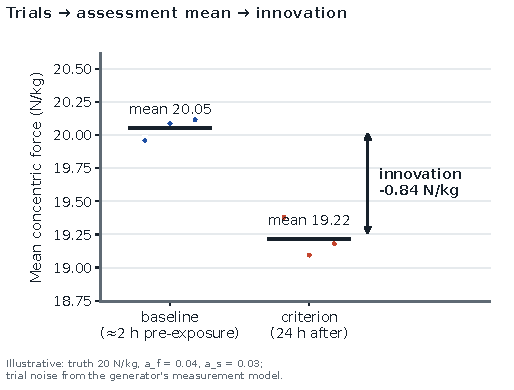
\includegraphics[width=\columnwidth]{figures/Fig3.pdf}\fi
\caption{Three-trial assessment and innovation. Trials are drawn with the simulator's measurement model around an illustrative baseline truth of \SI{20}{\Nkg} and a criterion truth shifted by the fixed-mode response at \SI{24}{\hour} ($a_f=0.04$, $a_s=0.03$). The innovation is the difference of the two three-trial means, Eq.~\eqref{eq:innovation}.}
\label{fig:innovation}
\end{figure}

\section{Mathematical recovery models}
\subsection{Fixed-mode response of the synthetic generator}
For each outcome the generator sets the criterion truth to the baseline truth times $1+r(\tau)+\epsilon$, where $\tau$ is the time since exposure and $\epsilon$ is a bounded discrepancy. The response is
\begin{equation}
r(\tau) = -a_f\,e^{-\tau/\SI{24}{\hour}} - a_s\,e^{-\tau/\SI{84}{\hour}},
\label{eq:response}
\end{equation}
with fast amplitude $a_f\in[0.01,0.08]$ and slow amplitude $a_s\in[0,0.08]$ (fractions of baseline). The \SI{24}{\hour} and \SI{84}{\hour} constants are fixed by the generator. They are \emph{mathematical modes chosen for the simulation}; they are not experimentally established recovery time constants, and the study makes no claim about biological timescales. Earlier exposure--response formulations such as the impulse--response and variable dose--response models \cite{Calvert1976,Busso2003} are related in spirit, but Eq.~\eqref{eq:response} is not a fit of either.

\subsection{Exposure, participants, camps and uncertainty}
The amplitudes arise from a sigmoid of a score built from normalized exposure axes (derived from eight current-exposure fields), four participant sensitivities and camp offsets. Participant sensitivities are the hyperbolic tangent of a linear map of four centered participant-context values plus normal residuals (standard deviation 0.45). Camp offsets have a logit standard deviation of 0.12, so effects are correlated within a camp and participant. A bounded smooth shared discrepancy (amplitude fraction 0.006, 32 random Fourier features) and a per-episode discrepancy (0.0030--0.0080) perturb the nominal modes. Forecast horizons are \SI{24}{\hour}, \SI{48}{\hour} and \SI{72}{\hour} after exposure (\Fig{fig:response}). Because the world is generated, the true response is known to the simulator, but it is hidden from every model.

\EvidenceFigure{figures/Fig4.pdf}{Fixed response modes of the synthetic generator (Eq.~\ref{eq:response}). (a) Illustrative amplitudes $a_f=0.04$, $a_s=0.03$; the vertical lines mark the three forecast horizons. (b) Envelope over the generator's amplitude support. These curves are synthetic assumptions and not observed recovery.}{fig:response}

\section{Neural architectures}
Nine original model families, M0--M8, were designed to forecast the two innovations from a common set of inputs: 39 raw features, an array of four prior episodes with four values each, the forecast horizon, and five public-schedule basis values. Each family has two recorded repeats (r0, r1), giving 18 routes. The families add structure cumulatively (Table~\ref{tab:arch}, \Fig{fig:arch}).
\begin{itemize}\setlength{\itemsep}{0pt}
\item \textbf{M0--M2} are feedforward networks on the raw features only, with exact GELU activations \cite{Hendrycks2016} and 1,346, 2,690 and 6,850 parameters.
\item \textbf{M3} adds a pointwise encoder of the four prior episodes with mean and latest pooling.
\item \textbf{M4} replaces it with a gated recurrent unit (GRU) \cite{Cho2014} reading the history in order.
\item \textbf{M5} adds a learned embedding of the forecast horizon.
\item \textbf{M6--M8} add the public-schedule basis: two values (M6), five values (M7), and a bias-free linear head from the five values to the two outputs (M8).
\end{itemize}
The basis is a fixed nominal construction from the known schedule of exposures (decays of \SI{36}{\hour} and \SI{120}{\hour} and a saturating total-dose transform). Its constants are a design choice of the architectures and are not the generator's \SI{24}{\hour} and \SI{84}{\hour} modes. Parameter counts rise from 1,346 to 10,796. The GRU accounts for most of the growth from M3 (7,138) to M4 (10,626); the horizon and basis stages (M5--M8) each add between 10 and 80 parameters. Outputs are additive innovations in \si{\Nkg} and \si{\mps}.

\EvidenceFigure{figures/Fig5.pdf}{Original architecture families M0--M8 and exact parameter counts from the model-qualification summary. The figure shows structure only; it reports no predictive performance, and none of these networks was scored in the public experiment.}{fig:arch}

\begin{table*}[!t]
\centering
\small\setlength{\tabcolsep}{3pt}\begin{tabularx}{\textwidth}{@{}lrlX@{}}
\toprule
Family & Parameters & Inputs & Structure \\
\midrule
M0 & 1,346 & 39 raw features & 39 $\to$ 32 $\to$ 2; exact GELU \\
M1 & 2,690 & 39 raw features & 39 $\to$ 64 $\to$ 2; exact GELU \\
M2 & 6,850 & 39 raw features & 39 $\to$ 64 $\to$ 64 $\to$ 2; exact GELU \\
M3 & 7,138 & 39 raw + 4 $\times$ 4 history & Raw backbone + pointwise history encoder; mean/latest pooling $\to$ 128 $\to$ 2 \\
M4 & 10,626 & 39 raw + 4 $\times$ 4 history & Raw backbone + 4 $\to$ 32 GRU; mean/latest pooling $\to$ 128 $\to$ 2 \\
M5 & 10,658 & 39 raw + 4 $\times$ 4 history + horizon & M4 + 2 $\times$ 8 horizon embedding $\to$ 136 $\to$ 2 \\
M6 & 10,738 & 39 raw + 4 $\times$ 4 history + horizon + 5 basis values & M5 + first two basis values $\to$ 16 $\to$ 152 $\to$ 2 \\
M7 & 10,786 & 39 raw + 4 $\times$ 4 history + horizon + 5 basis values & M5 + all five basis values $\to$ 16 $\to$ 152 $\to$ 2 \\
M8 & 10,796 & 39 raw + 4 $\times$ 4 history + horizon + 5 basis values & M7 + bias-free 5 $\to$ 2 linear basis head \\
\bottomrule
\end{tabularx}

\caption{Architecture contracts for the nine original families. Both repeats of each family share the parameter count shown. Original weights are not distributed.}
\label{tab:arch}
\end{table*}

Because the nine families and the four public reference models differ in targets, grids and evidence, no sentence in this paper attaches a public NRMSE to M0--M8. The architectures illustrate how the forecasting problem can be encoded; what they would achieve in a comparable experiment is unknown here.

\section{Synthetic experiment}
\subsection{Design reported with ADEMP}
We follow the ADEMP structure for simulation studies \cite{Morris2019}.

\emph{Aims.} Describe prediction error of simple reference forecasters across two outcomes, three horizons and three evaluation populations from one generator.

\emph{Data-generating mechanism.} The fixed-mode generator of Section~3. The training stream has 96 camps (24,000 episodes, 72,000 horizon rows) and the development stream 16 camps (4,000 episodes, 12,000 rows). Three evaluation roots, A, B and C, each have 16 camps, 4,000 episodes and 12,000 rows and are generated by the same generator from three fixed public seeds (\Fig{fig:design}). They are different seeds of one simulator, not independent cohorts. Participant, episode, query and camp identities are checked for separation between splits.

\emph{Estimand.} The baseline-relative innovations $\Delta F$ and $\Delta J$ at \SI{24}{\hour}, \SI{48}{\hour} and \SI{72}{\hour}: six cells.

\emph{Methods.} Each row has 82 public predictors (horizon, three baselines, two participant-context fields, eight current-exposure fields, and four prior episodes of 17 fields) that become 84 columns after one-hot horizon encoding. Labels, group keys, generator effects and oracle states are not predictors. Four reference models are evaluated: (1) zero innovation; (2) a training-mean constant per outcome and horizon; (3) ridge regression \cite{Hoerl1970} per cell with training-only scaling, the penalty selected on the development stream; (4) a structured comparator that multiplies normalized current-exposure primitives by the fixed \SI{24}{\hour} and \SI{84}{\hour} decay bases and adds baselines, participant context and prior-episode innovations, with coefficients estimated from training rows. Four ablations remove prior history, current exposure or participant context, and nested training subsets of 24, 48 and 96 camps are refit with the penalty held fixed.

\emph{Performance measures.} For each cell, RMSE divided by the population standard deviation of that cell's truth (NRMSE; a scale-free error in the sense of \cite{Hyndman2006}); the primary score is the equal-weight mean of the six cells. Uncertainty is a paired percentile bootstrap \cite{Efron1979} that resamples whole camps \cite{Cameron2008} (5,000 replicates, 16 camps), reported for each model's aggregate NRMSE and its difference from the zero baseline. With 16 clusters the intervals are descriptive and coarse.

\EvidenceFigure{figures/Fig6.pdf}{Design of the public synthetic experiment: one square is one camp (250 episodes, 750 horizon rows). Training (96 camps), development (16) and three evaluation roots (16 each) share one generator; an episode's three queries stay in one split. The predictor set excludes keys, labels and hidden effects.}{fig:design}

\section{Quantitative results}
\subsection{Six-cell error across models and roots}
Table~\ref{tab:overall} gives the mean six-cell NRMSE. The zero baseline scored 2.430659, the training mean 1.036038, ridge regression 0.736270 and the structured comparator 0.773316. A value near 1 means the model's error is comparable to the spread of the truth. The training mean is near that level by construction, and both fitted models are well below it. Differences between roots were small (standard deviations 0.003--0.008), consistent with the three roots sharing one generator; they quantify seed variation and not external validity.

\begin{table}[!t]
\centering
\footnotesize\setlength{\tabcolsep}{3pt}\begin{tabular*}{\columnwidth}{@{\extracolsep{\fill}}lrrr}
\toprule
Model & Mean & SD across roots & Range \\
\midrule
Zero innovation & 2.430659 & 0.008127 & 2.4213--2.4355 \\
Training mean & 1.036038 & 0.007308 & 1.0278--1.0417 \\
Ridge regression & 0.736270 & 0.003349 & 0.7327--0.7394 \\
Structured comparator & 0.773316 & 0.005490 & 0.7676--0.7785 \\
\bottomrule
\end{tabular*}

\caption{Mean six-cell NRMSE across the three evaluation roots, with the sample standard deviation and range across roots. These are descriptive synthetic results for the four evaluated reference models.}
\label{tab:overall}
\end{table}

By cell (\Fig{fig:perf}, Fig.~\ref{fig:heat}, Table~\ref{tab:cells}), ridge error increased with horizon, from 0.6244 (force) and 0.6522 (impulse) at \SI{24}{\hour} to 0.8157 and 0.8336 at \SI{72}{\hour}. Impulse error exceeded force error at every horizon for both fitted models. The zero baseline moved the other way, from 3.0335 to 2.1090 for force, consistent with a larger innovation at short lags. The decreasing amplitude of the fixed modes with lag is consistent with fitted-model skill falling as signal shrinks relative to noise and discrepancy; we did not test this explanation.

\EvidenceFigure{figures/Fig7.pdf}{Six-cell NRMSE for the four evaluated reference models. Each panel is one outcome (columns) and horizon (rows); colors mark the model, markers the evaluation root and the black line the three-root mean. The dashed line marks NRMSE $=1$.}{fig:perf}

\begin{table}[!t]
\centering
\footnotesize\setlength{\tabcolsep}{3pt}\begin{tabular*}{\columnwidth}{@{\extracolsep{\fill}}lrrrrrr}
\toprule
Model & F24 & F48 & F72 & J24 & J48 & J72 \\
\midrule
Zero innovation & 3.034 & 2.542 & 2.109 & 2.762 & 2.264 & 1.873 \\
Training mean & 1.048 & 1.039 & 1.027 & 1.045 & 1.032 & 1.025 \\
Ridge regression & 0.624 & 0.732 & 0.816 & 0.652 & 0.760 & 0.834 \\
Structured comparator & 0.658 & 0.761 & 0.843 & 0.696 & 0.805 & 0.878 \\
\bottomrule
\end{tabular*}

\caption{Mean NRMSE per cell across the three roots. F: mean concentric-force innovation (\si{\Nkg}); J: net-impulse innovation (\si{\mps}); the number is the horizon in hours.}
\label{tab:cells}
\end{table}

\EvidenceFigure{figures/Fig8.pdf}{Model-by-cell heatmap of mean NRMSE. Values are the stored across-root means.}{fig:heat}

\subsection{Recorded uncertainty}
Table~\ref{tab:int} lists the recorded camp-bootstrap intervals (\Fig{fig:boot}). In each root, the interval for the aggregate NRMSE of ridge lay below that of the structured comparator, and the paired difference from the zero baseline was entirely negative for both fitted models (for example, ridge in root A: $[-1.7522,-1.6450]$). Every recorded comparison is with the zero baseline. No paired interval for ridge versus the structured comparator was recorded, and none is computed here, so we describe ridge as lower in each root without claiming a tested difference.

\begin{table}[!t]
\centering
\footnotesize\setlength{\tabcolsep}{3pt}\begin{tabular*}{\columnwidth}{@{\extracolsep{\fill}}llrr}
\toprule
Root & Model & NRMSE 95\% interval & Difference from zero \\
\midrule
A & Ridge & [0.7280, 0.7462] & [-1.7522, -1.6450] \\
A & Structured & [0.7638, 0.7843] & [-1.7147, -1.6081] \\
B & Ridge & [0.7338, 0.7453] & [-1.7156, -1.6484] \\
B & Structured & [0.7735, 0.7846] & [-1.6766, -1.6092] \\
C & Ridge & [0.7264, 0.7401] & [-1.7338, -1.6691] \\
C & Structured & [0.7612, 0.7751] & [-1.7005, -1.6325] \\
\bottomrule
\end{tabular*}

\caption{Recorded paired camp-bootstrap 95\% percentile intervals (5,000 valid replicates, 16 camps per root) for aggregate NRMSE and its difference from the zero baseline (negative favors the model).}
\label{tab:int}
\end{table}

\EvidenceFigure{figures/Fig9.pdf}{Recorded camp-bootstrap intervals by root. Intervals are descriptive, rely on 16 camps, and compare models with the zero baseline only.}{fig:boot}

\subsection{Ablations and nested training camps}
Removing prior history raised ridge NRMSE from 0.736270 to 0.819681 and removing current exposure raised it to 0.867735, whereas removing participant context changed it by only 0.000076 (Table~\ref{tab:abl}). For the structured comparator, removing prior history raised NRMSE from 0.773316 to 0.820342. In this generator, therefore, current exposure and history carried the usable signal. In the nested diagnostic (Table~\ref{tab:nested}, \Fig{fig:abl}) ridge NRMSE changed from 0.736889 at 24 camps to 0.736270 at 96; the structured comparator from 0.773624 to 0.773316. Twenty-four camps already contain 6,000 episodes. All selected penalties equal 0.01, the lower edge of the frozen grid, so weaker regularization remains an open question for a separately specified study.

\begin{table}[!t]
\centering
\footnotesize\setlength{\tabcolsep}{3pt}\begin{tabular*}{\columnwidth}{@{\extracolsep{\fill}}lrr}
\toprule
Variant & Mean NRMSE & $\Delta$ vs full \\
\midrule
Ridge, full & 0.736270 & -- \\
Ridge, without prior history & 0.819681 & +0.083411 \\
Ridge, without current exposure & 0.867735 & +0.131465 \\
Ridge, without participant context & 0.736346 & +0.000076 \\
Structured, full & 0.773316 & -- \\
Structured, without prior history & 0.820342 & +0.047026 \\
\bottomrule
\end{tabular*}

\caption{Ablations, mean NRMSE across roots.}
\label{tab:abl}
\end{table}
\begin{table}[!t]
\centering
\footnotesize\setlength{\tabcolsep}{3pt}\begin{tabular*}{\columnwidth}{@{\extracolsep{\fill}}lrrr}
\toprule
Training camps & Ridge & Structured & Training mean \\
\midrule
24 & 0.736889 & 0.773624 & 1.038164 \\
48 & 0.736602 & 0.773621 & 1.037354 \\
96 & 0.736270 & 0.773316 & 1.036038 \\
\bottomrule
\end{tabular*}

\caption{Nested training-camp diagnostics, mean NRMSE across roots, with the penalty held fixed.}
\label{tab:nested}
\end{table}

\EvidenceFigure{figures/Fig10.pdf}{Ablations and nested training-camp results.}{fig:abl}

\section{Discussion}
\textbf{What the controlled results show.} On this generator, simple fitted linear forecasters recover a substantial part of the innovation variance at all three horizons, and most of the benefit comes from knowing the current exposure and recent history. Skill fell with horizon, and impulse was harder to predict than force. The structured comparator, which builds in the generator's fixed modes, did not outperform unconstrained ridge regression. Possible reasons are that its restricted basis cannot absorb participant-specific amplitudes and the shared discrepancy, or that the freely fitted features capture shape the nominal modes do not; both are hypotheses and we have no experiment that separates them.

\textbf{Architecture choices.} The nine original families encode a sensible progression: raw features, order-aware history, horizon awareness and a schedule-based basis. That progression is a design rationale. Whether the GRU, horizon embedding or basis stages improve forecasts could be tested only in a new, pre-specified comparison on the same data with the same scoring; this paper does not provide one, and the reference-model ablations should not be read as evidence about the networks. One transferable observation is that in the reference models the history and exposure inputs mattered much more than participant context, which suggests where architectural capacity would plausibly be most useful on this generator.

\textbf{Meaning of the synthetic findings.} The results depend on assumptions that are untestable against athletes: that recovery is a two-mode decay, that amplitudes are bounded, and that noise is as specified. A different generator could reverse the ranking of ridge and the structured comparator. The results support statements about this simulated forecasting task and about the behavior of the evaluated methods; they do not support statements about human recovery.

\section{Reproducibility and source identity}\label{sec:repro}
All numbers in this paper are read from the public receipts of the fixed-mode reference study (scientific-results SHA-256 \texttt{25032133\ldots20e4bc71}; protocol SHA-256 \texttt{972733eb\ldots{}a7838f48}) and the public model-qualification summary. The source release is v1.1.0. Figures and tables are regenerated by the scripts in this package with no training, fitting, inference or scoring.

Supporting verification concerns the original architectures. A recovered reference implementation reproduces the original CPU predictions exactly for all 18 routes. Agreement with archived GPU arrays is within the recorded tolerance for M0--M3 (8 of 18 routes) and outside it for M4--M8 (10 of 18 routes) (\Fig{fig:num}), a difference in numerical environment rather than a scientific finding. Original checkpoints and weights are private, no public checkpoint replay is promised, and these checks establish numerical reproducibility of recovered routes only. The retrospective reconstruction of the original research from archived material is the subject of a separate companion article.

\EvidenceFigure{figures/Fig11.pdf}{Numerical qualification of the 18 recovered routes against original CPU outputs and archived GPU arrays. This supports reproducibility of the architectures and says nothing about their predictive accuracy.}{fig:num}

\section{Limitations}
\begin{itemize}\setlength{\itemsep}{0pt}
\item All data are simulated by one generator; no athlete was measured, so predictive validity for real recovery is not established.
\item The 24-hour and 84-hour modes, amplitude bounds, noise levels and the half-sine trial are modeling assumptions, not measured quantities.
\item The three evaluation roots differ only by seed; they measure seed variation, not generalization to other populations or generators.
\item Intervals resample 16 camps per root, compare with the zero baseline only, and are descriptive. No ridge-versus-structured comparison, significance test or multiplicity adjustment is made.
\item Nine original networks were not scored in the public experiment; no conclusion about their relative accuracy is offered.
\item Selected ridge and structured penalties sit at the lower grid edge.
\item The force--time pulse is a simulator choice; real CMJ waveforms, event detection, filtering and instrument error are outside the study.
\item Numerical qualification concerns recovered routes; GPU differences for M4--M8 are unresolved and checkpoints are private.
\item This is an owner-review draft: it has not been peer reviewed, submitted, or assigned a DOI, and a human domain review of the cited literature is pending.
\end{itemize}

\section{Conclusions}
A CMJ's gross mean concentric force and net impulse, referenced to a baseline, give two innovations whose post-exposure change can be modeled with simple mathematical response modes and forecast with learned models. In a controlled synthetic benchmark, two fitted reference models reduced six-cell NRMSE from 2.43 (zero innovation) and 1.04 (training mean) to 0.74 and 0.77, with current exposure and prior history carrying most of the signal and little sensitivity to training-set size beyond 24 camps. These findings concern the synthetic forecasting task. Whether the nine original architectures, or any model, would forecast real recovery remains untested.

\section*{Data, code and availability}
The public synthetic results, architecture summary, figure and table scripts and receipts are in the repository release v1.1.0 and this package. Row-level datasets are regenerated from public seeds and are not committed. Original checkpoints are private. Author names, affiliations, roles, funding and conflict statements remain to be confirmed by the owner.

\bibliographystyle{plos2025}
\bibliography{bibliography/references}
\end{document}
